% Provenance (never printed): see sources/outline_sources.md (Year 3: refraction and
% reflection seismic methods; CMP acquisition, NMO, stacking, Dix; migration in
% principle; seismic stratigraphy). Brief: sources/book5/BRIEFS.md, ch. 2. Curves from
% figdata/bachelor-3/seismic_model.py, refraction_dip.py, synthetic_seismogram.py,
% cmp_nmo.py (the Varden column, region.py); exercise and problem values in the
% Book 5 scratch calculator calc/ch02.py.
\chapter{Seismologi Eksplorasi}\label{ch:b3:exploration-seismology}

Sebuah kapal survei bergerak perlahan sepanjang garis lurus di laut, menarik susunan
air gun beberapa meter di bawah permukaan dan, di belakangnya, kabel
sepanjang beberapa kilometer yang dilengkapi hidrofon. Dalam satu survei yang diuraikan kepada
regulator, susunan itu menampung \num{5240} inci kubik udara terkompresi, ditembakkan setiap
\qty{8}{s} dari kedalaman \qty{12}{m} di bawah permukaan, dan streamer azimut sempit
di belakang kapal semacam itu merekam offset 8 sampai \qty{10}{km}.
% ledger: noaa5:wg-survey
Setiap tembakan mengirimkan denyut bunyi ke dasar laut, dan setiap antarmuka batuan
di bawahnya memantulkan gema samar. Beberapa minggu setelah pemrosesan, seorang geolog menelusuri
penampang yang memperlihatkan alur sungai terkubur, blok sesar miring, dan
pengisian \omterm{def:b3:exploration-seismology:terminations}{onlap} cekungan tua tampak seolah tanah itu dibelah terbuka.
Seismologi skala Bumi pada bab sebelumnya memakai gelombang
gempa bumi; seismologi eksplorasi membuat gelombangnya sendiri, dengan sumber yang waktu dan
tempatnya diketahui persis, dan merekamnya pada ribuan kanal. Bab ini
mengikuti gema dari tembakan sampai penampang: survei refraksi,
refleksi wavelet oleh kolom berlapis, metode \omterm{def:b3:exploration-seismology:cmp}{titik tengah bersama}
yang mengubah gema berulang menjadi kecepatan dan citra yang bersih, migrasi, yang
mengembalikan reflektor ke tempatnya, dan pembacaan penampang sebagai
stratigrafi.

\begin{recall}
Pada batas antara dua medium dengan impedansi akustik $Z_1 = \rho_1v_1$ dan
$Z_2 = \rho_2v_2$, gelombang bidang pada datang tegak lurus dipantulkan dengan
koefisien amplitudo $R = (Z_2 - Z_1)/(Z_2 + Z_1)$ (volume Tahun 2
buku fisika, tentang gelombang pada antarmuka). Gelombang kepala, waktu intersep, dan
jarak silang profil refraksi di atas lapisan datar telah dibahas pada
volume Tahun 1, pada bab tentang Bumi berlapis; log lubang bor di Buku 2
kelas 11). Konvolusi $(f*g)(t) = \int f(\tau)g(t - \tau)\,\mathrm d\tau$
dan transformasi Fourier berasal dari buku matematika. \omterm{def:b3:seismology-imaging:ray-parameter}{Parameter sinar} dan
\omterm{def:b3:seismology-imaging:inverse}{masalah invers} linear dibahas pada \cref{ch:b3:seismology-imaging}.
\end{recall}

\section{Survei refraksi}

\begin{definition}[Survei refraksi dan refleksi seismik]\label{def:b3:exploration-seismology:surveys}
Yang disebut \emph{survei refraksi seismik}\index{survei refraksi seismik} merekam, sepanjang
satu garis penerima, waktu datang pertama dari sumber terkontrol, dan menggunakan
gelombang kepala yang merambat di sepanjang bagian atas lapisan yang lebih cepat untuk menentukan kecepatan dan
kedalamannya. Sementara itu, \emph{survei refleksi seismik}\index{survei refleksi seismik}
merekam seluruh rangkaian gelombang, pada offset yang kebanyakan lebih kecil daripada
yang diminati, dan menggunakan gelombang yang dipantulkan pada datang hampir tegak lurus oleh
antarmuka untuk mencitrakan perlapisan.
\end{definition}

Di atas lapisan datar, gelombang kepala tiba pada $t = x/v_2 + t_i$, sebuah garis lurus
yang gradiennya memberikan kecepatan $v_2$ refraktor dan intersepnya $t_i$
memberikan kedalamannya. Refraktor yang miring membuat garis itu miring: gelombang kepala dari tembakan
searah kemiringan datang makin lama makin terlambat seiring refraktor makin dalam, dan tampak lambat;
ditembakkan berlawanan arah kemiringan, tampak cepat. Dengan menembak dua arah sepanjang garis yang sama, profil terbalik
memisahkan kecepatan dari kemiringannya.

\begin{theorem}[Refraksi pada antarmuka miring]\label{thm:b3:exploration-seismology:dipping}
Sebuah lapisan dengan kecepatan $v_1$ berada di atas refraktor bidang berkecepatan $v_2 > v_1$ yang miring
dengan sudut $\theta$ sepanjang profil; $i_c = \arcsin(v_1/v_2)$, dan $h$ adalah
kedalaman tegak lurus refraktor di bawah tembakan. Di luar jarak kritis
gelombang kepala tiba pada
\begin{align*}
  t &= \frac{x\sin(i_c + \theta)}{v_1} + \frac{2h\cos i_c}{v_1}
  &&\text{searah kemiringan},\\
  t &= \frac{x\sin(i_c - \theta)}{v_1} + \frac{2h\cos i_c}{v_1}
  &&\text{berlawanan arah kemiringan}.
\end{align*}
Kecepatan semu $v_d = v_1/\sin(i_c + \theta)$ dan
$v_u = v_1/\sin(i_c - \theta)$ dari profil terbalik memberikan
\[
  i_c = \tfrac12\left[\arcsin\frac{v_1}{v_d} + \arcsin\frac{v_1}{v_u}\right],\qquad
  \theta = \tfrac12\left[\arcsin\frac{v_1}{v_d} - \arcsin\frac{v_1}{v_u}\right],
  \qquad v_2 = \frac{v_1}{\sin i_c} .
\]
\end{theorem}

\begin{proof}
Putar kerangka sehingga refraktor mendatar; permukaan lalu miring dengan
$\theta$, dan untuk tembakan searah kemiringan, kedalaman tegak lurus di bawah penerima pada
offset $x$ adalah $h + x\sin\theta$, proyeksinya pada refraktor
$x\cos\theta$. Lintasan gelombang kepala turun pada sudut kritis $i_c$ menuju
normal, sepanjang refraktor dengan $v_2$, dan naik pada $i_c$. Waktunya adalah
\[
  t = \frac{h}{v_1\cos i_c} + \frac{x\cos\theta - h\tan i_c - (h + x\sin\theta)\tan i_c}{v_2}
  + \frac{h + x\sin\theta}{v_1\cos i_c}.
\]
Dengan $1/v_2 = \sin i_c/v_1$ dan $1/\cos i_c - \sin i_c\tan i_c = \cos i_c$,
suku-suku dengan $h$ memberikan $2h\cos i_c/v_1$ dan yang dengan $x$ memberikan
$x(\sin i_c\cos\theta + \cos i_c\sin\theta)/v_1 = x\sin(i_c + \theta)/v_1$.
Berlawanan arah kemiringan, $\theta$ berganti tanda. Rumus terakhir membalik kedua
kecepatan semu.
\end{proof}

Kedua cabang profil terbalik harus memberikan waktu yang sama antara kedua
titik tembak, dari ujung mana pun ditembakkan: \emph{waktu resiprokal}, pemeriksaan atas
pemilihan waktu tiba. Dua situasi menggagalkan metode ini. Lapisan yang lebih lambat
dari lapisan di atasnya (inversi kecepatan) tidak membiaskan gelombang kepala dan tak terlihat: batuannya
dihitung dalam lapisan di atasnya, dan setiap kedalaman di bawahnya dilebihkan. Lapisan
yang lebih cepat dari lapisan di atasnya tetapi terlalu tipis mungkin tidak pernah memberikan waktu tiba pertama, karena
gelombang kepala lapisan yang lebih dalam dan lebih cepat menyusulnya: lapisan tersembunyi. Survei
refleksi melihat keduanya.

\begin{omfigure}
\begin{tikzpicture}
\begin{axis}[omrecord, width=0.82\linewidth, height=0.46\linewidth,
  xmin=0, xmax=1200, ymin=0, ymax=660,
  xlabel={posisi sepanjang bentangan, dari tembakan B (\unit{m})},
  ylabel={waktu (\unit{ms})}, legend pos=north west, legend cell align=left,
  legend style={font=\scriptsize}]
\addplot[gray, thick, densely dashed] table[x=x, y=tdir] {figdata/out/bachelor-3-refraction_dip-west.dat};
\addlegendentry{gelombang langsung ($v_1$)}
\addplot[blue!70!black, thick] table[x=x, y=thead] {figdata/out/bachelor-3-refraction_dip-west.dat};
\addlegendentry{gelombang kepala dari B, ke atas kemiringan}
\addplot[red!70!black, thick] table[x expr=1200-\thisrow{x}, y=thead] {figdata/out/bachelor-3-refraction_dip-east.dat};
\addlegendentry{gelombang kepala dari T, ke bawah kemiringan}
\addplot[gray, thick, densely dashed, forget plot] table[x expr=1200-\thisrow{x}, y=tdir] {figdata/out/bachelor-3-refraction_dip-east.dat};
\addplot[only marks, mark=*, mark size=1.5pt] coordinates {(1200,486.13) (0,486.13)};
\node[font=\scriptsize, anchor=south east] at (axis cs:1190,530) {waktu resiprokal};
\end{axis}
\end{tikzpicture}

\par\smallskip{\small Profil refraksi terbalik pada sayap barat
antiklin Varden (hasil hitungan; soal, Bagian I). Refraktor, yakni puncak
batu gamping, naik dari barat ke timur dengan sudut \ang{10.8} di bawah bentangan \qty{1200}{m};
kapur dan serpih di atasnya digabung menjadi satu lapisan dengan kecepatan \qty{2.40}{km.s^{-1}}. Gelombang
kepala dari tembakan di barat, berlawanan arah kemiringan, tampak cepat (\qty{6.57}{km.s^{-1}}),
sedangkan yang dari timur, searah kemiringan, lambat (\qty{3.52}{km.s^{-1}}); keduanya memerlukan \qty{486.1}{ms} untuk
menempuh seluruh bentangan. Gelombang kepala baru menyusul gelombang langsung hanya di dekat
ujung jauh: refraktor ini dalam untuk bentangan yang sependek itu.}
\label{fig:b3:exploration-seismology:refraction}
\end{omfigure}

\section{Refleksi pada sudut datang normal}

\begin{definition}[Wavelet seismik, wavelet Ricker]\label{def:b3:exploration-seismology:wavelet}
Yang disebut \emph{wavelet seismik}\index{wavelet seismik} adalah pulsa pendek, beberapa puluh
milidetik lamanya, yang dikirim sumber dan sistem perekam melalui
tanah; setiap reflektor memantulkan salinan terskalanya. Adapun \emph{wavelet
Ricker}\index{wavelet Ricker} dengan frekuensi puncak $f$ adalah pulsa fase-nol
\[
  w(t) = \left(1 - 2\pi^2f^2t^2\right)e^{-\pi^2f^2t^2},
\]
turunan kedua fungsi Gauss dengan pengecualian tanda dan skalanya: puncak pusat dan
dua lobus samping, dengan rata-rata nol dan spektrum amplitudo yang memuncak pada $f$.
\end{definition}

\begin{definition}[Deret reflektivitas]\label{def:b3:exploration-seismology:synthetic}
Suatu \emph{deret reflektivitas}\index{deret reflektivitas} dari kolom berlapis adalah
deret koefisien refleksi sudut datang normal $r_k$ dari bidang antarmukanya,
diletakkan pada waktu vertikal dua arahnya $\tau_k = \sum_{i \le k} 2h_i/v_i$:
$r(t) = \sum_k r_k\,\delta(t - \tau_k)$.
\end{definition}

\begin{proposition}[Model konvolusi]\label{prop:b3:exploration-seismology:synthetic}
Jika hanya pantulan primer yang dipertahankan (tanpa kelipatan), pada sudut datang normal, dengan
tanpa kehilangan transmisi, atenuasi, atau penyebaran, dan wavelet $w$ tidak
berubah terhadap kedalaman, jejak yang terekam adalah konvolusi wavelet dengan
\omterm{def:b3:exploration-seismology:synthetic}{deret reflektivitas}:
\[
  s(t) = \sum_k r_k\,w(t - \tau_k) = (w*r)(t) .
\]
Jejak yang dihitung dengan cara ini dari log lubang bor kecepatan dan massa jenis adalah
\emph{seismogram sintetik}\index{seismogram sintetik} dari log tersebut.
\end{proposition}

\begin{proof}
Setiap bidang antarmuka memantulkan salinan wavelet datang yang diskalakan oleh koefisiennya
dan tertunda sesuai waktu dua arahnya; perekamannya linear, sehingga salinan-salinan itu dijumlahkan.
Jumlah itu adalah konvolusi $w$ dengan deretan impuls Dirac berbobot
$r(t)$, karena $w*\delta(\cdot - \tau_k) = w(\cdot - \tau_k)$.
\end{proof}

\omterm{prop:b3:exploration-seismology:synthetic}{Seismogram sintetik} adalah cara sebuah sumur bor dikaitkan dengan penampang seismik: sebuah
refleksi pada penampang dicocokkan dengan bidang antarmuka pada log yang menghasilkannya.
Kolom Varden di bawah sumbu sinklin soal (model seismik bab ini,
dengan kecepatan dan massa jenis yang dipilih dalam rentang terbitan untuk
setiap batuan)
% ledger: mavko:velocities
menghasilkan gambar di bawah. Bidang antarmuka kapur--serpih hanya memantulkan
\qty{2.8}{\percent} amplitudo, karena kapur dan serpih kebetulan memiliki
impedansi yang hampir sama; puncak batu gamping memantulkan \qty{38}{\percent},
dasar batu gamping mengembalikan pulsa terbalik, dan batuan dasar
memantulkan pulsa positif yang kuat.

\begin{omfigure}
\begin{tikzpicture}
\begin{groupplot}[group style={group size=3 by 1, horizontal sep=0.45cm, y descriptions at=edge left},
  width=0.36\linewidth, height=0.6\linewidth, y dir=reverse, ymin=0.4, ymax=0.85,
  tick label style={font=\scriptsize}, label style={font=\small}, title style={font=\small}]
\nextgroupplot[title={impedansi}, xlabel={\scriptsize $10^6$\,\unit{kg.m^{-2}.s^{-1}}},
  ylabel={waktu dua arah (\unit{s})}, xmin=4, xmax=14]
\addplot[black, thick] table[x=imp, y=t] {figdata/out/bachelor-3-synthetic_seismogram-log.dat};
\node[font=\tiny, anchor=west] at (axis cs:5.1,0.45) {kapur};
\node[font=\tiny, anchor=west] at (axis cs:5.4,0.535) {serpih};
\node[font=\tiny, anchor=east] at (axis cs:11.6,0.62) {batu gamping};
\node[font=\tiny, anchor=west] at (axis cs:7.0,0.70) {batu pasir};
\node[font=\tiny, anchor=east] at (axis cs:13.1,0.79) {sekis};
\nextgroupplot[title={reflektivitas}, xmin=-0.45, xmax=0.45, xtick={-0.4,0,0.4}]
\addplot[xcomb, red!70!black, thick, mark=*, mark size=1.2pt] table[x=r, y=t] {figdata/out/bachelor-3-synthetic_seismogram-refl.dat};
\draw[gray] (axis cs:0,0.4) -- (axis cs:0,0.85);
\nextgroupplot[title={jejak sintetik}, xmin=-0.45, xmax=0.45, xtick={-0.4,0,0.4}]
\addplot[blue!70!black, thick] table[x=s, y=t] {figdata/out/bachelor-3-synthetic_seismogram-trace.dat};
\draw[gray] (axis cs:0,0.4) -- (axis cs:0,0.85);
\end{groupplot}
\end{tikzpicture}

\par\smallskip{\small \omterm{prop:b3:exploration-seismology:synthetic}{Seismogram sintetik} kolom Varden di bawah sumbu
sinklin (hasil hitungan). Kiri: impedansi setiap lapisan terhadap waktu dua
arah. Tengah: \omterm{def:b3:exploration-seismology:synthetic}{deret reflektivitas}, satu puncak per bidang antarmuka (batangnya mengarah
ke kanan untuk kenaikan impedansi). Kanan: konvolusinya dengan sebuah
\omterm{def:b3:exploration-seismology:wavelet}{wavelet Ricker} \qty{30}{Hz}. Setiap refleksi adalah salinan wavelet; refleksi kapur--serpih yang samar
pada \qty{0.488}{s}, hampir tidak terlihat.}
\label{fig:b3:exploration-seismology:synthetic}
\end{omfigure}

Seberapa tipis suatu lapisan yang masih dapat dibedakan refleksi? Puncak dan dasarnya
masing-masing memantulkan sebuah wavelet; jika keduanya bertumpang tindih, keduanya berinterferensi.

\begin{definition}[Ketebalan tuning]\label{def:b3:exploration-seismology:resolution}
Yang disebut \emph{ketebalan tuning}\index{ketebalan tuning} dari suatu lapisan adalah ketebalan
pada saat refleksi dari puncak dan dasarnya, yang berlawanan tanda, berinterferensi
paling konstruktif, sehingga amplitudo gabungannya paling besar. Lapisan yang lebih tipis
tidak terpisahkan: puncak dan dasarnya tidak lagi dapat dipilih secara terpisah, dan
amplitudo berkurang sebanding dengan ketebalannya.
\end{definition}

\begin{proposition}[Aturan seperempat panjang gelombang]\label{prop:b3:exploration-seismology:tuning}
Untuk wavelet dengan periode dominan $T$ dalam lapisan berkecepatan $v$, dengan
koefisien refleksi $+R$ di puncaknya dan $-R$ di dasarnya, refleksi gabungan
paling kuat ketika ketebalan lapisan $b = \lambda/4$, dengan $\lambda = vT$; untuk
$b \ll \lambda/4$ amplitudonya sebanding dengan $b$.
\end{proposition}

\begin{proof}
Nyatakan wavelet dengan harmonik dominannya $\cos(2\pi t/T)$. Kedua refleksi
tersebut adalah $R\cos(2\pi t/T) - R\cos(2\pi(t - \Delta t)/T)$ dengan
$\Delta t = 2b/v$, yang amplitudonya $2R|\sin(\pi\Delta t/T)|$: terbesar untuk
$\Delta t = T/2$, yaitu $b = vT/4$; untuk $\Delta t$ kecil nilainya kira-kira
$2\pi R\Delta t/T = 4\pi Rb/\lambda$.
\end{proof}

\omterm{def:b3:exploration-seismology:wavelet}{Wavelet Ricker} bukan harmonik, dan \omterm{def:b3:exploration-seismology:resolution}{ketebalan tuning-nya}, yang dibaca dari
model baji pada gambar di bawah, sedikit lebih kecil dari seperempat panjang
gelombang pada frekuensi puncak: \qty{19.5}{m} pada \qty{30}{Hz} di batuan berkecepatan
\qty{3000}{m.s^{-1}}, untuk $\lambda/4 = \qty{25}{m}$. Data seismik jarang memuat
energi berarti di atas beberapa puluh hertz dari kedalaman kilometer, sebab
batuan menyerap frekuensi tinggi; lapisan dengan tebal kurang dari sekitar \qty{20}{m}
tampak sebagai satu refleksi tunggal.

\begin{omfigure}
\begin{tikzpicture}
\begin{axis}[omrecord, width=0.74\linewidth, height=0.42\linewidth,
  xmin=0, xmax=80, ymin=0, ymax=1.8,
  xlabel={ketebalan lapisan $b$ (\unit{m})}, ylabel={amplitudo puncak / $R$}]
\addplot[blue!70!black, thick] table[x=b, y expr=2*\thisrow{amp}] {figdata/out/bachelor-3-synthetic_seismogram-wedge.dat};
\draw[red!70!black, densely dashed] (axis cs:19.5,0) -- (axis cs:19.5,1.6);
\node[font=\scriptsize, anchor=south, red!70!black] at (axis cs:19.5,1.6) {tuning, \qty{19.5}{m}};
\draw[gray, densely dotted] (axis cs:25,0) -- (axis cs:25,1.6);
\node[font=\scriptsize, anchor=west, gray!40!black] at (axis cs:25.5,0.3) {$\lambda/4 = \qty{25}{m}$};
\draw[gray] (axis cs:0,1) -- (axis cs:80,1);
\node[font=\scriptsize, anchor=south east] at (axis cs:79,1) {dua wavelet terpisah};
\end{axis}
\end{tikzpicture}

\par\smallskip{\small Model baji (dihitung): lapisan dengan
\qty{3000}{m.s^{-1}} dengan koefisien refleksi $+R$ di puncaknya dan $-R$ di
dasarnya, dicitrakan dengan \omterm{def:b3:exploration-seismology:wavelet}{wavelet Ricker} \qty{30}{Hz}. Amplitudo puncak dari
refleksi gabungan, relatif terhadap satu refleksi dengan koefisien $R$, naik linear dari nol
untuk lapisan yang sangat tipis, memuncak pada \omterm{def:b3:exploration-seismology:resolution}{ketebalan tuning}, lalu menetap
di tingkat dua wavelet terpisah untuk lapisan tebal.}
\label{fig:b3:exploration-seismology:wedge}
\end{omfigure}

Secara lateral, resolusi ditentukan oleh lebar reflektor yang
mengembalikan energi secara sefase.

\begin{definition}[Zona Fresnel]\label{def:b3:exploration-seismology:fresnel}
Yang disebut \emph{zona Fresnel}\index{zona Fresnel} (pertama) dari suatu reflektor, dengan
sumber dan penerima berimpit pada tinggi $z$ di atasnya, adalah cakram reflektor
di sekitar titik datang normal, tempat lintasan dua arah lebih panjang daripada
lintasan normal kurang dari setengah panjang gelombang: refleksinya tiba secara sefase dan
membentuk bersama-sama refleksi yang terekam.
\end{definition}

\begin{proposition}[Jari-jari zona Fresnel]\label{prop:b3:exploration-seismology:fresnel}
\omterm{def:b3:exploration-seismology:fresnel}{Zona Fresnel} pertama memiliki jari-jari
$r_F = \sqrt{\lambda z/2 + \lambda^2/16} \approx \sqrt{\lambda z/2}$ untuk
$\lambda \ll z$.
\end{proposition}

\begin{proof}
Titik pada reflektor yang berjarak $r$ dari titik datang normal berada
pada jarak $\sqrt{z^2 + r^2}$ dari sumber. Kelebihan lintasan dua arahnya adalah
$2(\sqrt{z^2 + r^2} - z)$; dengan menyamakannya dengan $\lambda/2$ diperoleh
$\sqrt{z^2 + r^2} = z + \lambda/4$, sehingga $r^2 = \lambda z/2 + \lambda^2/16$.
\end{proof}

Pada kedalaman \qty{1}{km}, dengan $\lambda = \qty{100}{m}$, \omterm{def:b3:exploration-seismology:fresnel}{zona Fresnel} berjari-jari
\qty{225}{m}: fitur yang lebih sempit dari itu tersamar, kecuali
migrasi (dijelaskan di bawah) memadatkan zona tersebut.

\begin{omfigure}
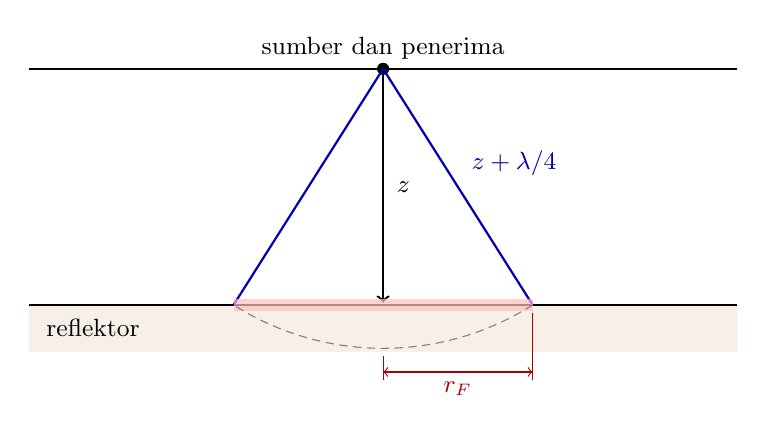
\begin{tikzpicture}[font=\small, x=1cm, y=1cm]
\fill[brown!12] (-4.5,-3.6) rectangle (4.5,-3.0);
\draw[thick] (-4.5,-3.0) -- (4.5,-3.0);
\node[anchor=north west] at (-4.4,-3.05) {reflektor};
\draw[thick] (-4.5,0) -- (4.5,0);
\fill (0,0) circle (2.2pt) node[above] {sumber dan penerima};
\draw[->, thick] (0,0) -- (0,-2.97);
\node[anchor=west] at (0.05,-1.5) {$z$};
\draw[blue!70!black, thick] (0,0) -- (1.9,-3.0);
\draw[blue!70!black, thick] (0,0) -- (-1.9,-3.0);
\node[anchor=west, blue!70!black] at (1.0,-1.2) {$z + \lambda/4$};
\fill[red!25, opacity=0.7] (-1.9,-3.08) rectangle (1.9,-2.92);
\draw[red!70!black] (0,-3.65) -- (0,-3.95) (1.9,-3.1) -- (1.9,-3.95);
\draw[<->, red!70!black] (0,-3.85) -- (1.9,-3.85) node[midway, below] {$r_F$};
\draw[gray, densely dashed] (-57.6:3.55) arc (-57.6:-122.4:3.55);
\end{tikzpicture}

\par\smallskip{\small \omterm{def:b3:exploration-seismology:fresnel}{Zona Fresnel} pertama (skematis): bagian dari
reflektor yang jaraknya dari sumber dan penerima yang berimpit melebihi
jarak normal $z$ kurang dari $\lambda/4$ (busur putus-putus: bola berjari-jari
$z + \lambda/4$), sehingga kelebihan lintasan dua arah kurang dari setengah panjang gelombang
dan pantulannya tiba secara sefase. Skala $\lambda$ dibesar-besarkan.}
\label{fig:b3:exploration-seismology:fresnel}
\end{omfigure}

\section{Akuisisi dan pemrosesan titik tengah bersama}

Satu pantulan terlalu lemah untuk terlihat di tengah derau. Oleh karena itu, survei refleksi
merekam setiap titik bawah permukaan berkali-kali, dengan pasangan sumber--penerima yang berbeda,
lalu menjumlahkan rekamannya.

\begin{definition}[Titik tengah bersama, liputan]\label{def:b3:exploration-seismology:cmp}
Untuk sumber di $x_s$ dan penerima di $x_r$ pada suatu garis, titik tengahnya adalah
$(x_s + x_r)/2$ dan offset $x = |x_r - x_s|$. Yang disebut \emph{titik
tengah bersama}\index{titik tengah bersama} (CMP) adalah kumpulan jejak dari semua
tembakan yang memakai titik tengah yang sama; pada lapisan datar semuanya memantul dari
titik bawah permukaan yang sama. Yang disebut \emph{liputan}\index{liputan}
adalah jumlah jejak dalam satu kumpulan. Dengan $N$ kanal pada
interval penerima $\Delta g$ dan satu tembakan setiap $\Delta s$ sepanjang garis, liputannya
adalah $N\Delta g/(2\Delta s)$.
\end{definition}

\begin{omfigure}
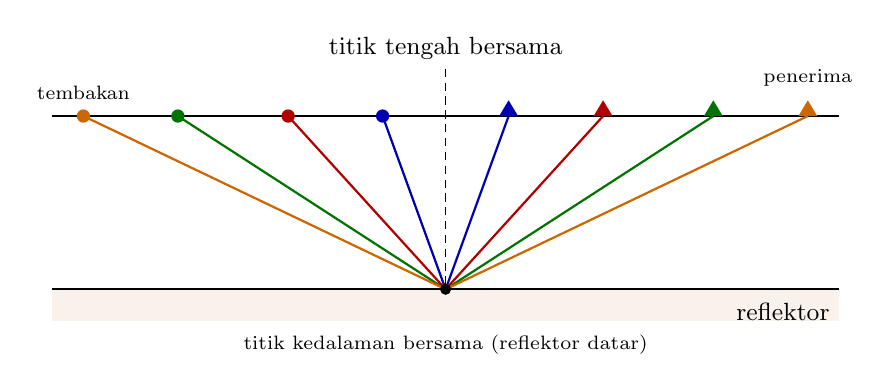
\begin{tikzpicture}[font=\small, x=1cm, y=1cm]
\draw[thick] (-5,0) -- (5,0);
\fill[brown!10] (-5,-2.6) rectangle (5,-2.2);
\draw[thick] (-5,-2.2) -- (5,-2.2);
\node[anchor=north east] at (5,-2.25) {reflektor};
\foreach \off/\col in {0.8/blue!70!black, 2.0/red!70!black, 3.4/green!45!black, 4.6/orange!80!black} {
  \draw[\col, thick] (-\off,0) -- (0,-2.2) -- (\off,0);
  \fill[\col] (-\off,0) circle (2.4pt);
  \fill[\col] (\off-0.12,0) -- (\off+0.12,0) -- (\off,0.2) -- cycle;
}
\fill (0,-2.2) circle (2pt);
\draw[densely dashed] (0,0.6) -- (0,-2.2);
\node[anchor=south] at (0,0.6) {titik tengah bersama};
\node[anchor=north, align=center, font=\scriptsize] at (0,-2.65) {titik kedalaman bersama (reflektor datar)};
\node[anchor=south, font=\scriptsize] at (-4.6,0.08) {tembakan};
\node[anchor=south, font=\scriptsize] at (4.6,0.25) {penerima};
\end{tikzpicture}

\par\smallskip{\small Geometri \omterm{def:b3:exploration-seismology:cmp}{titik tengah bersama} (skematis): empat pasangan sumber--penerima
(titik, segitiga) dengan offset berbeda berbagi titik tengah yang sama; di atas
reflektor datar, semuanya memantul dari titik yang sama di bawahnya. Jejaknya membentuk
kumpulan dengan \omterm{def:b3:exploration-seismology:cmp}{liputan} empat.}
\label{fig:b3:exploration-seismology:cmp}
\end{omfigure}

\begin{theorem}[Moveout normal]\label{thm:b3:exploration-seismology:nmo}
Pada lapisan berkecepatan $v$ di atas reflektor datar pada waktu tempuh vertikal dua arah
$t_0$, refleksi yang terekam pada offset $x$ tiba pada
\[
  t(x)^2 = t_0^2 + \frac{x^2}{v^2},
\]
berupa hiperbola pada bidang $(x, t)$. Selisih $\Delta t = t(x) - t_0$ disebut
\emph{moveout normal}\index{moveout normal}; untuk $x \ll vt_0$,
$\Delta t \approx x^2/(2v^2t_0)$.
\end{theorem}

\begin{proof}
Lintasan refleksi bergerak dari sumber ke titik refleksi di bawah
titik tengah lalu naik kembali ke penerima: dua kaki dengan panjang
$\sqrt{(vt_0/2)^2 + (x/2)^2}$. Jadi $t = (2/v)\sqrt{(vt_0/2)^2 + (x/2)^2}$ dan
$t^2 = t_0^2 + x^2/v^2$. Lalu $t - t_0 = (t^2 - t_0^2)/(t + t_0) \approx
x^2/(2v^2t_0)$.
\end{proof}

Pada beberapa lapisan, waktu refleksi tidak lagi tepat hiperbolik, namun
kira-kira demikian pada offset kecil, dengan kecepatan yang merupakan rata-rata terbobot dari
lapisan-lapisan.

\begin{definition}[Stacking, kecepatan akar kuadrat rata-rata, dan kecepatan interval]\label{def:b3:exploration-seismology:velocities}
Yang disebut \emph{kecepatan interval}\index{kecepatan interval} $v_i$ suatu lapisan adalah
kecepatannya sendiri; dengan $\Delta t_i = 2h_i/v_i$ sebagai waktu tempuh dua arah melintasinya, maka
\emph{kecepatan akar kuadrat rata-rata}\index{kecepatan akar kuadrat rata-rata} hingga ke
dasar lapisan $n$ adalah
\[
  V_{\text{rms},n} = \left(\frac{\sum_{i\le n}v_i^2\,\Delta t_i}{\sum_{i\le n}\Delta t_i}\right)^{1/2}.
\]
Yang disebut \emph{kecepatan stacking}\index{kecepatan stacking} dari suatu refleksi adalah
kecepatan $V$ dari hiperbola $t^2 = t_0^2 + x^2/V^2$ yang paling sesuai dengan waktu-waktunya dalam
kumpulan CMP.
\end{definition}

\begin{proposition}[Kecepatan stacking pada offset kecil]\label{prop:b3:exploration-seismology:rms}
Pada lapisan datar, $t(x)^2 = t_0^2 + x^2/V_{\text{rms}}^2 + O(x^4)$: untuk offset
kecil, \omterm{def:b3:exploration-seismology:velocities}{kecepatan stacking} adalah \omterm{def:b3:exploration-seismology:velocities}{kecepatan akar kuadrat rata-rata}.
\end{proposition}

\begin{proof}
Untuk \omterm{def:b3:seismology-imaging:ray-parameter}{parameter sinar} $p$, $x = \sum_i 2h_i\tan\varphi_i$ dan
$t = \sum_i 2h_i/(v_i\cos\varphi_i)$, dengan $\sin\varphi_i = pv_i$. Pada orde kedua
dalam $p$, $\tan\varphi_i \approx pv_i$ dan $1/\cos\varphi_i \approx 1 +
p^2v_i^2/2$, jadi $x \approx p\sum v_i^2\Delta t_i = pV_{\text{rms}}^2t_0$ dan
$t \approx t_0 + \tfrac12p^2V_{\text{rms}}^2t_0$. Maka
$t^2 \approx t_0^2 + p^2V_{\text{rms}}^2t_0^2 = t_0^2 + x^2/V_{\text{rms}}^2$, dengan
suku-suku yang diabaikan berorde $p^4$, yaitu $x^4$.
\end{proof}

\begin{theorem}[Persamaan Dix]\label{thm:b3:exploration-seismology:dix}
Jika $V_{n-1}$ dan $V_n$ adalah \omterm{def:b3:exploration-seismology:velocities}{kecepatan akar kuadrat rata-rata} hingga ke puncak dan dasar lapisan
$n$, pada waktu dua arah $t_{n-1}$ dan $t_n$, \omterm{def:b3:exploration-seismology:velocities}{kecepatan interval}
lapisan itu diberikan oleh \emph{persamaan Dix}\index{persamaan Dix}
\[
  v_n^2 = \frac{V_n^2t_n - V_{n-1}^2t_{n-1}}{t_n - t_{n-1}} ,
\]
dan tebalnya adalah $h_n = v_n(t_n - t_{n-1})/2$.
\end{theorem}

\begin{proof}
Menurut definisi $V_n^2t_n = \sum_{i\le n}v_i^2\Delta t_i$ dan $V_{n-1}^2t_{n-1}
= \sum_{i\le n-1}v_i^2\Delta t_i$. Selisihnya adalah $v_n^2\Delta t_n$, dengan
$\Delta t_n = t_n - t_{n-1}$.
\end{proof}

Analisis kecepatan memindai setiap kumpulan untuk mencari hiperbola yang paling sesuai dengan
energi: untuk setiap percobaan $t_0$ dan $V$, jejak dijumlahkan sepanjang kurva, dan
ukuran koherensi (kemiripan) dipetakan; analis memilih nilai maksimumnya,
reflektor demi reflektor, untuk membangun fungsi kecepatan. Koreksi NMO kemudian
menggeser setiap sampel pada setiap jejak dari $t(x)$ ke $t_0$, sehingga refleksinya
menjadi datar, dan jejak setiap kumpulan dijumlahkan.

\begin{definition}[Stacking]\label{def:b3:exploration-seismology:stack}
Yang disebut \emph{stacking}\index{stacking} adalah penjumlahan, setelah
koreksi \omterm{thm:b3:exploration-seismology:nmo}{moveout normal}, dari jejak-jejak sebuah kumpulan CMP menjadi satu jejak
yang diletakkan pada titik tengah. Jejak hasil stacking, berjajar sepanjang garis, membentuk
penampang stacking, citra reflektor dalam waktu dua arah.
\end{definition}

\begin{proposition}[Penguatan hasil stacking]\label{prop:b3:exploration-seismology:sqrtN}
Jika $N$ jejak sebuah kumpulan memuat sinyal refleksi yang sama dan derau yang saling bebas
dengan simpangan baku $\sigma$ yang sama, rata-ratanya memuat sinyal yang sama
dan derau dengan simpangan baku $\sigma/\sqrt N$: \omterm{def:b3:exploration-seismology:stack}{stacking} menaikkan
rasio sinyal terhadap derau sebesar $\sqrt N$.
\end{proposition}

\begin{proof}
Varians jumlah $N$ peubah bebas adalah jumlah varians-variansnya,
$N\sigma^2$; dibagi $N^2$, rata-ratanya memiliki varians
$\sigma^2/N$ (simpangan baku rata-rata, yang sudah dikenal dari
buku matematika).
\end{proof}

\begin{omfigure}
\begin{tikzpicture}
\begin{groupplot}[group style={group size=2 by 1, horizontal sep=0.5cm, y descriptions at=edge left},
  width=0.52\linewidth, height=0.56\linewidth, y dir=reverse, ymin=0.4, ymax=0.92,
  xmin=-150, xmax=2150, tick label style={font=\scriptsize}, title style={font=\small},
  xlabel={\scriptsize offset (\unit{m})}]
\nextgroupplot[title={(a) kumpulan CMP}, ylabel={waktu dua arah (\unit{s})}]
\addplot[black, very thin, unbounded coords=jump] table[x=x, y=t] {figdata/out/bachelor-3-cmp_nmo-gather-raw.dat};
\nextgroupplot[title={(b) setelah koreksi NMO}]
\addplot[black, very thin, unbounded coords=jump] table[x=x, y=t] {figdata/out/bachelor-3-cmp_nmo-gather-nmo.dat};
\end{groupplot}
\end{tikzpicture}

\par\smallskip{\small Kumpulan CMP sintetis di bawah sumbu sinklin
garis Varden (dihitung dengan penelusuran sinar eksak melalui kolom berlapis datar; 30
Hz, \omterm{def:b3:exploration-seismology:wavelet}{wavelet Ricker}, tanpa derau). (a) Keempat refleksi (puncak serpih, puncak
dan dasar batu gamping, puncak batuan dasar) melengkung turun seiring offset
sepanjang hampir-hiperbola. (b) Setelah koreksi NMO dengan \omterm{def:b3:exploration-seismology:velocities}{kecepatan stacking} yang
dicocokkan pada offset sampai \qty{600}{m}, refleksi menjadi datar hingga sekitar
\qty{1}{km}; di luar itu, waktu sebenarnya menyimpang dari hiperbola dan
koreksi membuatnya tetap melengkung, dan wavelet-nya meregang; dalam pemrosesan,
jejak jauh yang meregang dari refleksi dangkal dibisukan sebelum
\omterm{def:b3:exploration-seismology:stack}{stacking}.}
\label{fig:b3:exploration-seismology:gather}
\end{omfigure}

\begin{omfigure}
\begin{tikzpicture}
\begin{axis}[omrecord, width=0.72\linewidth, height=0.46\linewidth,
  xmin=0.4, xmax=0.78, ymin=2000, ymax=5000,
  xlabel={waktu dua arah $t_0$ (\unit{s})}, ylabel={kecepatan (\unit{m.s^{-1}})},
  legend cell align=left, legend columns=2,
  legend style={font=\scriptsize, at={(0.5,-0.24)}, anchor=north}]
\addplot[gray, thick, const plot mark right] table[x=t0, y=vint] {figdata/out/bachelor-3-cmp_nmo-vel.dat};
\addlegendentry{kecepatan interval model}
\addplot[gray, thick, forget plot] coordinates {(0.4,2500) (0.487847,2500)};
\addplot[blue!70!black, thick, mark=*, mark size=1.5pt] table[x=t0, y=vrms] {figdata/out/bachelor-3-cmp_nmo-vel.dat};
\addlegendentry{kecepatan RMS}
\addplot[red!70!black, only marks, mark=square*, mark size=1.6pt] table[x=t0, y=vstack] {figdata/out/bachelor-3-cmp_nmo-vel.dat};
\addlegendentry{kecepatan stacking (offset sampai \qty{600}{m})}
\addplot[green!45!black, only marks, mark=triangle*, mark size=2pt] table[x=t0, y=vdix] {figdata/out/bachelor-3-cmp_nmo-vel.dat};
\addlegendentry{kecepatan interval Dix}
\end{axis}
\end{tikzpicture}

\par\smallskip{\small Kecepatan di bawah sumbu sinklin (dihitung). Kecepatan RMS,
yaitu rata-rata berbobot, berubah perlahan; \omterm{def:b3:exploration-seismology:velocities}{kecepatan stacking} pada kumpulan itu
berada dekat dengannya. Jika diterapkan padanya, \omterm{thm:b3:exploration-seismology:dix}{persamaan Dix} memulihkan \omterm{def:b3:exploration-seismology:velocities}{kecepatan interval}
tiap lapisan (garis tangga, digambar di dasar tiap lapisan) hingga
dalam beberapa persen, dengan galat yang membesar pada batu gamping yang tipis dan cepat.}
\label{fig:b3:exploration-seismology:velocities}
\end{omfigure}

\begin{omfigure}
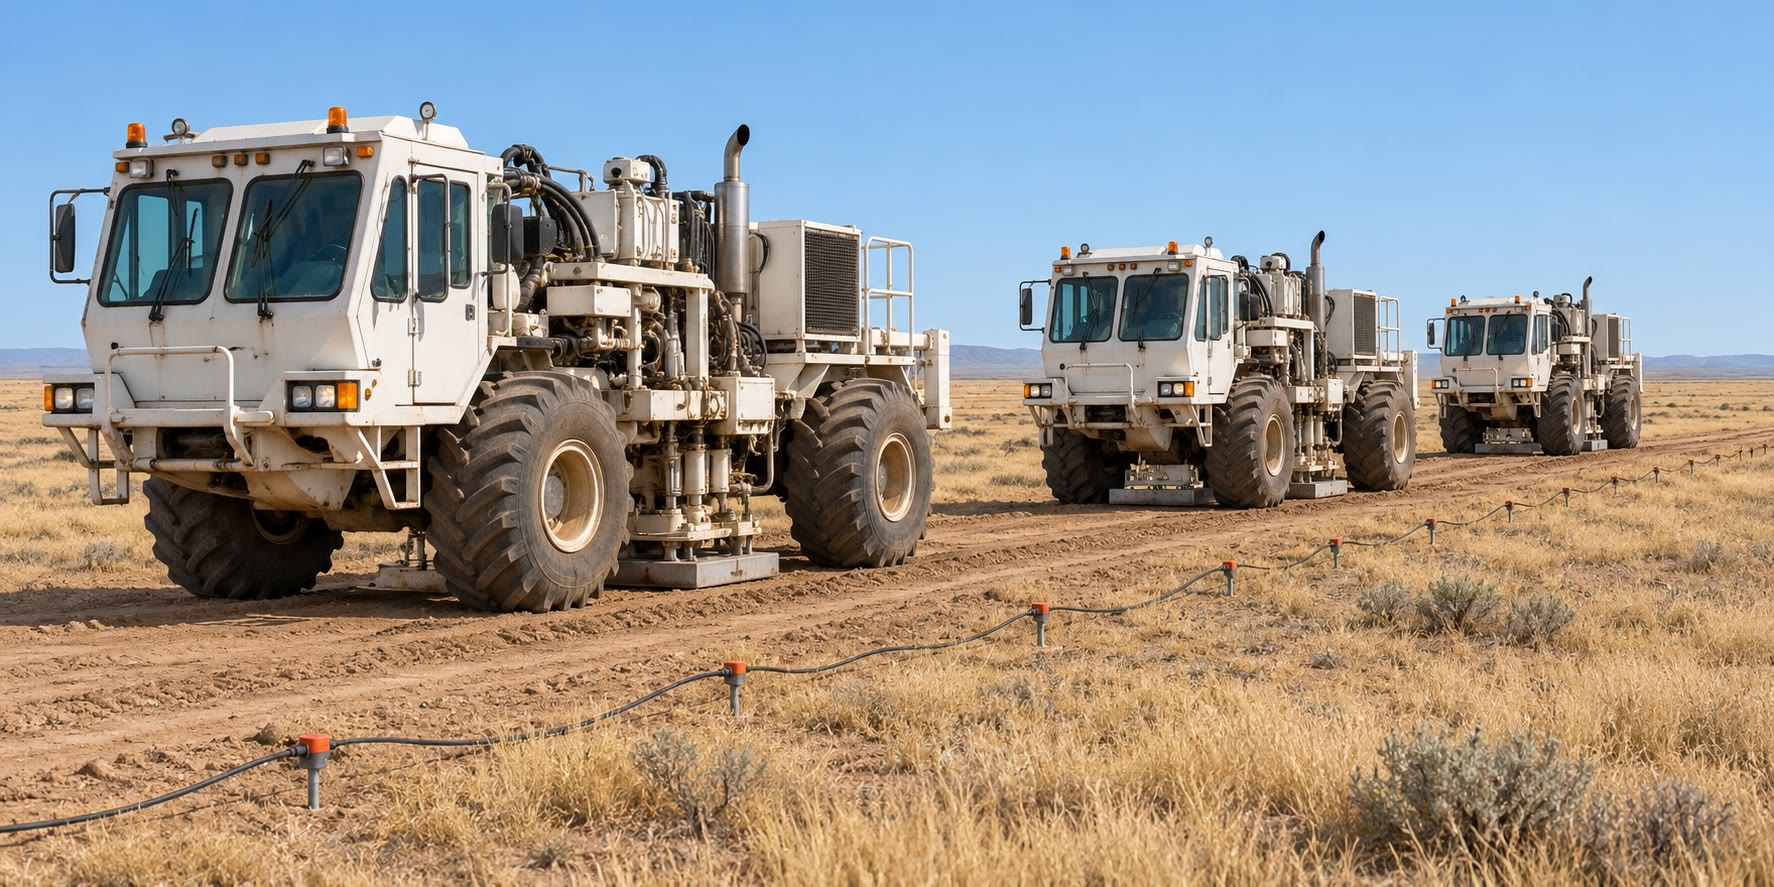
\includegraphics[width=0.62\linewidth]{images/book5/ai/b3-vibroseis.jpg}

\par\smallskip{\small Truk-truk vibrator pada garis survei darat: alih-alih
ledakan, tiap truk menekan pelat berat ke tanah dan menggetarkannya dengan
sapuan frekuensi selama beberapa detik; rekaman yang panjang dimampatkan
menjadi pulsa pendek dengan mengorelasikannya terhadap sapuan itu (ilustrasi buatan AI).}
\label{fig:b3:exploration-seismology:vibroseis}
\end{omfigure}

\section{Migrasi}

Penampang \omterm{def:b3:exploration-seismology:stack}{stacking} menunjukkan tiap refleksi di bawah titik tengah tempat ia
direkam, pada waktu yang dibutuhkan gema untuk kembali. Untuk reflektor datar,
posisinya memang di situ. Untuk reflektor miring tidak demikian: gema yang direkam di sebuah titik permukaan berasal
dari titik reflektor yang paling dekat dengannya, yang terletak naik-kemiringan,
bukan tegak lurus di bawahnya. Titik-titik seperti ujung pemotongan sesar, yang
menghamburkan energi ke segala arah, tampak sebagai hiperbola.

\begin{definition}[Migrasi seismik]\label{def:b3:exploration-seismology:migration}
Yang disebut \emph{migrasi seismik}\index{migrasi seismik} adalah langkah pemrosesan yang
memindahkan refleksi pada penampang seismik ke posisi reflektor
yang menghasilkannya: ia memulihkan kemiringan dan posisi sebenarnya reflektor yang miring
serta memampatkan hiperbola difraksi dari penghambur titik ke
puncaknya. Dilakukan dengan model kecepatan dalam waktu, ia menghasilkan penampang
termigrasi-waktu; dengan model dalam kedalaman, ia menghasilkan citra kedalaman.
\end{definition}

\begin{theorem}[Kemiringan pada penampang offset-nol]\label{thm:b3:exploration-seismology:dip}
Dalam medium berkecepatan $v$, sebuah reflektor bidang dengan kemiringan $\theta$ pada bidang
penampang tampak pada penampang offset-nol, diplot sebagai kedalaman $vt/2$
tegak lurus di bawah tiap titik rekam, sebagai garis dengan kemiringan semu $\theta_a$
dengan
\[
  \tan\theta_a = \sin\theta .
\]
Refleksi yang direkam di titik $x$ berasal dari titik reflektor yang berjarak
$(vt/2)\sin\theta$ naik-kemiringan dari titik yang tegak lurus di bawah $x$.
\end{theorem}

\begin{proof}
Sinar offset-nol tegak lurus terhadap reflektor, sehingga waktu yang direkam di $x$ adalah
$t = 2d(x)/v$, dengan $d(x)$ jarak dari $x$ ke bidang. Jarak itu
bertambah sebesar $\sin\theta$ untuk setiap satuan $x$ searah kemiringan, sehingga kedalaman yang diplot
$vt/2 = d(x)$ memiliki kemiringan $\sin\theta$. Kaki normal dari $x$
ke bidang terletak pada jarak horizontal $d\sin\theta$ dari $x$, di sisi
naik-kemiringan.
\end{proof}

Karena $\tan\theta_a = \sin\theta < \tan\theta$, penampang yang belum termigrasi selalu
menunjukkan kemiringan yang lebih landai daripada yang sebenarnya, dan tidak dapat
menunjukkan kemiringan yang lebih curam daripada \ang{45} sama sekali. Penghambur titik pada kedalaman $z$ di bawah titik $x_0$ kembali di
$x$ dengan waktu offset-nol $t(x) = (2/v)\sqrt{z^2 + (x - x_0)^2}$: sebuah hiperbola dengan
puncaknya tepat di atas titik itu, yaitu difraksinya. Migrasi dalam bentuk paling sederhananya,
yaitu \omterm{def:b3:exploration-seismology:stack}{stacking} difraksi, menjumlahkan tiap penampang sepanjang hiperbola difraksi dari
setiap penghambur yang mungkin dan meletakkan jumlahnya di puncak: reflektor, yang merupakan
garis kontinu dari penghambur, muncul di tempat sebenarnya, dan
difraksi-difraksi itu terkumpul.

\begin{omfigure}
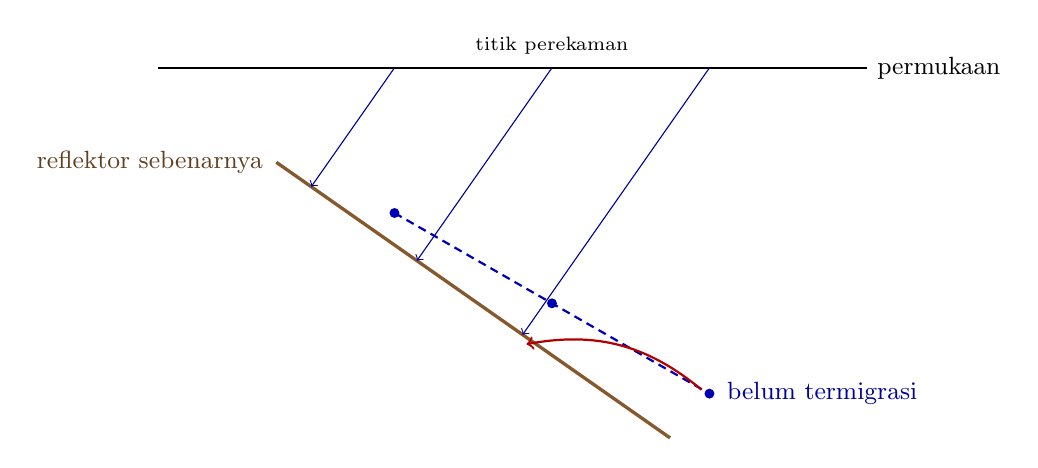
\begin{tikzpicture}[font=\small, x=1cm, y=1cm]
 \draw[thick] (-0.5,0) -- (8.5,0) node[right] {permukaan};
% true reflector, dip 35 deg, rising to the left
\draw[very thick, brown!70!black] (1.0,-1.2) -- (6.0,-4.70);
\node[brown!50!black, anchor=east] at (0.95,-1.2) {reflektor sebenarnya};
% zero-offset normal rays from x = 2, 4, 6
\foreach \x in {2.5, 4.5, 6.5} {
  % distance from (x,0) to the line through (1,-1.2) dir (cos35,-sin35): normal n=(sin35,cos35)
  \pgfmathsetmacro{\dd}{abs(0.5736*(\x-1.0) + 0.8192*(0+1.2))}
  \draw[blue!60!black, ->] (\x,0) -- ++({-0.5736*\dd},{-0.8192*\dd});
  \fill[blue!70!black] (\x,{-\dd}) circle (1.8pt);
}
% apparent reflector through the plotted points
\pgfmathsetmacro{\da}{abs(0.5736*1.5 + 0.8192*1.2)}
\pgfmathsetmacro{\db}{abs(0.5736*5.5 + 0.8192*1.2)}
\draw[blue!70!black, thick, densely dashed] (2.5,{-\da}) -- (6.5,{-\db});
\node[blue!60!black, anchor=west] at (6.6,{-\db}) {belum termigrasi};
\node[anchor=south, font=\scriptsize] at (4.5,0.05) {titik perekaman};
\draw[->, red!70!black, thick] (6.4,{-\db+0.05}) to[bend right=25] ({6.5-0.5736*\db+0.05},{-0.8192*\db-0.12});
\end{tikzpicture}

\par\smallskip{\small Migrasi reflektor yang miring (skematis, kemiringan sebenarnya
\ang{35}). Sinar offset-nol di setiap titik perekaman tegak lurus terhadap
reflektor, sehingga gemanya berasal dari arah naik-kemiringan; diplot secara vertikal di bawah titik,
pada kedalaman $vt/2$, refleksi tampak lebih landai (garis putus-putus: $\tan\theta_a =
\sin\theta$, di sini \ang{29.8}), dan bergeser ke arah turun-kemiringan. Migrasi (panah merah) memindahkannya kembali.}
\label{fig:b3:exploration-seismology:migration}
\end{omfigure}

\section{Stratigrafi seismik}

Penampang yang sudah termigrasi adalah gambaran perlapisan, dan ia dapat dibaca sebagai
stratigrafi: refleksi mengikuti permukaan perlapisan, yang merupakan
garis waktu, sehingga geometrinya mencatat bagaimana cekungan itu terisi.

\begin{definition}[Stratigrafi seismik, fasies seismik]\label{def:b3:exploration-seismology:seismic-stratigraphy}
Yang disebut \emph{stratigrafi seismik}\index{stratigrafi seismik} adalah interpretasi
stratigrafi dan sejarah pengendapan suatu cekungan dari geometri
refleksi seismiknya. Sebuah \emph{fasies seismik}\index{fasies seismik} adalah satuan
tiga dimensi refleksi yang karakternya (kemenerusan, amplitudo,
frekuensi, geometri internal: sejajar, divergen, sigmoid, kacau, membukit)
berbeda dari satuan tetangganya dan diinterpretasikan sebagai lingkungan
pengendapan.
\end{definition}

\begin{definition}[Terminasi refleksi]\label{def:b3:exploration-seismology:terminations}
Yang disebut \emph{terminasi refleksi}\index{terminasi refleksi} adalah akhir sebuah
refleksi yang menumpu pada refleksi lain. \emph{onlap}\index{onlap}: refleksi yang mula-mula horizontal
berakhir pada permukaan yang naik lebih curam, dengan lapisan yang lebih muda
menumpang pada lereng yang lebih tua. \emph{downlap}\index{downlap}: refleksi miring
berakhir ke arah turun-kemiringan pada permukaan yang lebih landai, ketika ujung-ujung
lapisan progradasi bertumpu di dasar cekungan. \emph{toplap}\index{toplap}: refleksi miring
berakhir ke arah naik-kemiringan pada permukaan di atasnya, dengan sedikit erosi, saat
puncak lapisan progradasi bertemu dengan muka laut. \emph{pemancungan
erosional}\index{pemancungan erosional}: refleksi berakhir ke arah naik-kemiringan pada
permukaan di atasnya yang memotongnya, yaitu ketidakselarasan.
\end{definition}

\begin{omfigure}
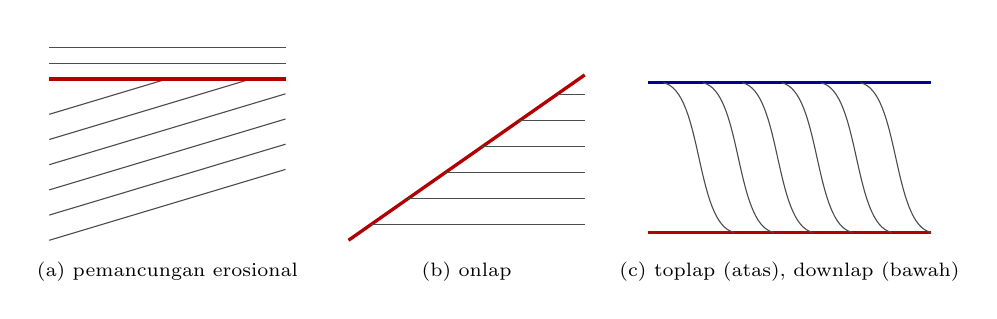
\begin{tikzpicture}[font=\scriptsize, x=1cm, y=1cm]
% erosional truncation: tilted beds cut by an unconformity
\begin{scope}
\foreach \k in {0,...,5} {\draw[gray!60!black] (0,{-2.3+0.32*\k}) -- (3.0,{-1.4+0.32*\k-0.25*0});}
\fill[white] (0,-0.25) -- (3.2,-0.25) -- (3.2,0.4) -- (0,0.4) -- cycle;
\draw[very thick, red!70!black] (0,-0.25) -- (3.0,-0.25);
\foreach \k in {0,1} {\draw[gray!60!black] (0,{-0.05+0.2*\k}) -- (3.0,{-0.05+0.2*\k});}
\node[anchor=north] at (1.5,-2.45) {(a) pemancungan erosional};
\end{scope}
% onlap
\begin{scope}[xshift=3.8cm]
\draw[very thick, red!70!black] (0,-2.3) -- (3.0,-0.2);
\foreach \k in {0,...,5} {\pgfmathsetmacro{\y}{-2.1+0.33*\k} \pgfmathsetmacro{\xe}{(\y+2.3)/0.7} \draw[gray!60!black] (\xe,\y) -- (3.0,\y);}
\node[anchor=north] at (1.5,-2.45) {(b) onlap};
\end{scope}
% downlap and toplap: clinoforms
\begin{scope}[xshift=7.6cm]
\draw[very thick, red!70!black] (0,-2.2) -- (3.6,-2.2);
\draw[very thick, blue!60!black] (0,-0.3) -- (3.6,-0.3);
\foreach \k in {0,...,5} {\draw[gray!60!black] ({0.2+0.5*\k},-0.3) .. controls ({0.7+0.5*\k},-0.4) and ({0.6+0.5*\k},-2.1) .. ({1.1+0.5*\k},-2.2);}
\node[anchor=north] at (1.8,-2.45) {(c) toplap (atas), downlap (bawah)};
\end{scope}
\end{tikzpicture}

\par\smallskip{\small \omterm{def:b3:exploration-seismology:terminations}{Terminasi refleksi} (penampang skematis, refleksi abu-abu,
permukaan terminasi berwarna). (a) Refleksi yang miring dipotong oleh
ketidakselarasan. (b) Refleksi datar yang berakhir pada lereng yang lebih tua. (c) Lapisan miring
dari baji progradasi yang berakhir ke arah naik-kemiringan pada permukaan di atasnya (\omterm{def:b3:exploration-seismology:terminations}{toplap}) dan
ke arah turun-kemiringan di dasar cekungan (\omterm{def:b3:exploration-seismology:terminations}{downlap}).}
\label{fig:b3:exploration-seismology:terminations}
\end{omfigure}

Terminasi-terminasi itu menandai permukaan yang membatasi rangkaian lapisan yang berhubungan secara genetik;
pemetaannya di seluruh cekungan, serta mengaitkannya dengan naik dan turunnya
muka laut relatif, adalah stratigrafi sekuen, yang dibahas dalam
\cref{ch:b3:sequence-stratigraphy}. Penampang seismik tepi pasif
umumnya memperlihatkan baji refleksi yang berprogradasi ke arah laut dan yang \omterm{def:b3:exploration-seismology:terminations}{downlap} ke
dasar laut dalam, ditutup oleh \omterm{def:b3:exploration-seismology:terminations}{toplap}, dan terkubur ke arah darat di bawah lapisan yang \omterm{def:b3:exploration-seismology:terminations}{onlap}, yang diendapkan
saat muka laut naik kembali.

\begin{inthefield}[Survei streamer laut dan tim darat]
\begin{minipage}[t]{0.55\linewidth}\vspace{0pt}
Pada survei laut kapal tidak pernah berhenti: ia berlayar lintasan demi lintasan dengan kecepatan beberapa
knot, larik air-gun menembak pada interval tetap, dan streamer dijaga pada
kedalaman tetap oleh sayap kecil yang dapat dikemudikan, dan posisinya ditentukan dengan akustik serta
penentuan posisi dengan satelit. Pengamat di anjungan memantau laut di sekitar larik, dan
survei bekerja berdasarkan aturan yang memuat langkah untuk melindungi mamalia laut,
jaga yang dilakukan dan apa yang dilaporkan.
% ledger: noaa5:itr-gom
Di darat, tim menggelar kabel atau unit perekam nirkabel di sepanjang lintasan;
truk vibrator bergerak beriringan dari satu titik sumber ke titik berikutnya, dan
truk perekam memeriksa setiap kanal sebelum setiap sapuan. Di pusat pengolahan
rekaman diurutkan menjadi kumpulan \omterm{def:b3:exploration-seismology:cmp}{titik tengah bersama}, kecepatan
dipilih, data \omterm{def:b3:exploration-seismology:stack}{di-stacking} dan dimigrasi, lalu penampang diserahkan kepada
para interpreter.
\end{minipage}\hfill
\begin{minipage}[t]{0.42\linewidth}\vspace{0pt}
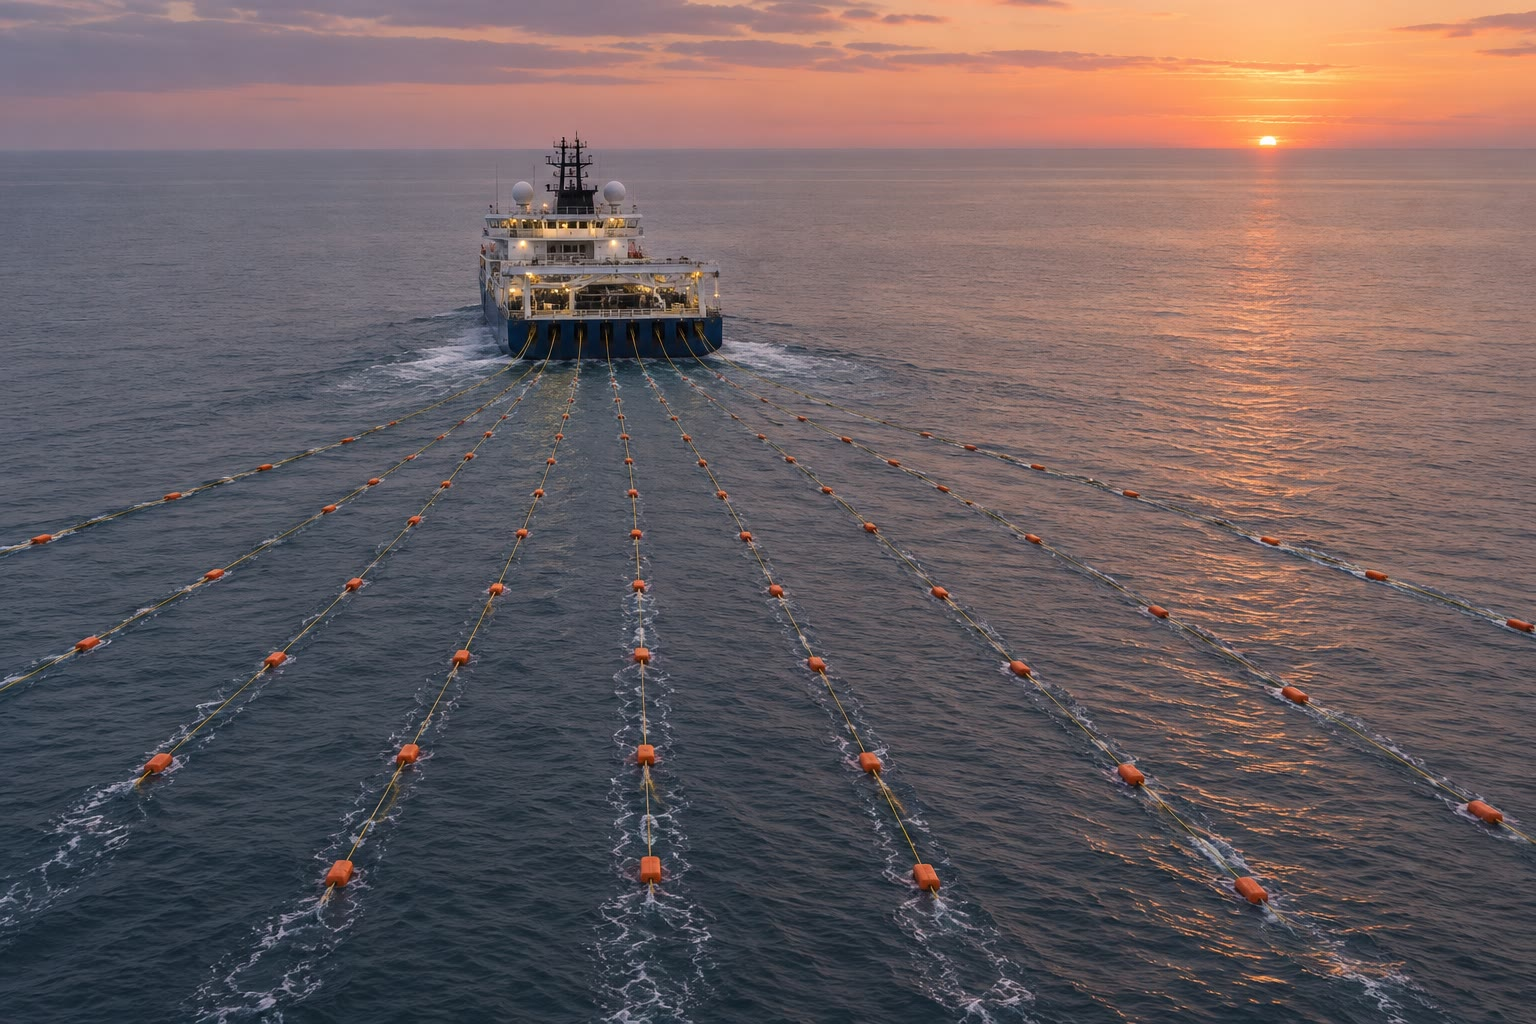
\includegraphics[width=\linewidth]{images/book5/ai/b3-streamer-vessel.jpg}

{\scriptsize Kapal survei seismik yang menarik streamer-nya saat senja
(ilustrasi buatan AI).}
\end{minipage}
\end{inthefield}

\section{Latihan}

\begin{exercise}[$\star$]\label{exo:b3:exploration-seismology:1}
Batu kapur ($v = \qty{2500}{m.s^{-1}}$, $\rho = \qty{2.00}{g.cm^{-3}}$) terletak di atas serpih
(\qty{2300}{m.s^{-1}}, \qty{2.30}{g.cm^{-3}}), yang terletak di atas batu gamping
(\qty{4500}{m.s^{-1}}, \qty{2.60}{g.cm^{-3}}). Hitung ketiga impedansi dan
koefisien refleksi kedua bidang batas. Berapa bagian dari energi datang
yang dipantulkan oleh puncak batu gamping?
% ledger: mavko:velocities
\end{exercise}

\begin{exercise}[$\star$]\label{exo:b3:exploration-seismology:2}
Reflektor datar terletak \qty{800}{m} di bawah lapisan berkecepatan \qty{2000}{m.s^{-1}}.
Hitung $t_0$, waktu refleksi pada offset \qty{1000}{m}, dan \omterm{thm:b3:exploration-seismology:nmo}{moveout normal}
di titik tersebut. Bandingkan dengan pendekatan $x^2/(2v^2t_0)$.
\end{exercise}

\begin{exercise}[$\star$]\label{exo:b3:exploration-seismology:3}
Sebuah streamer memiliki 240 kanal berjarak \qty{12.5}{m}, dan kapal menembak setiap
\qty{25}{m}. Hitung interval CMP dan \omterm{def:b3:exploration-seismology:cmp}{liputannya}. Berapa interval tembakan
yang memberikan \omterm{def:b3:exploration-seismology:cmp}{liputan} 120?
\end{exercise}

\begin{exercise}[$\star$]\label{exo:b3:exploration-seismology:4}
Dengan frekuensi dominan \qty{30}{Hz}, hitung panjang gelombang dan
seperempat panjang gelombang di batu pasir dengan \qty{3000}{m.s^{-1}} dan di batu gamping dengan
\qty{4500}{m.s^{-1}}. Hitung jari-jari \omterm{def:b3:exploration-seismology:fresnel}{zona Fresnel} pertama dari sebuah
reflektor yang berada \qty{1000}{m} di bawah batuan dengan kecepatan rata-rata \qty{2800}{m.s^{-1}}.
\end{exercise}

\begin{exercise}[$\star\star$]\label{exo:b3:exploration-seismology:5}
Dua refleksi memiliki $t_0 = \qty{0.500}{s}$ dengan \omterm{def:b3:exploration-seismology:velocities}{kecepatan akar kuadrat rata-rata}
\qty{2400}{m.s^{-1}}, dan $t_0 = \qty{0.700}{s}$ dengan \qty{2800}{m.s^{-1}}.
Hitung \omterm{def:b3:exploration-seismology:velocities}{kecepatan interval} dan ketebalan lapisan di antara keduanya.
\end{exercise}

\begin{exercise}[$\star\star$]\label{exo:b3:exploration-seismology:6}
Reflektor bidang memiliki kemiringan $\varphi$ pada bidang lintasan CMP, di dalam lapisan dengan
kecepatan $v$. (a) Tunjukkan bahwa $t(x)^2 = t_0^2 + x^2\cos^2\varphi/v^2$, dengan $t_0$ adalah
waktu offset-nol di titik tengah. (Petunjuk: gunakan bayangan titik tengah terhadap
reflektor.) (b) Turunkan \omterm{def:b3:exploration-seismology:velocities}{kecepatan stacking}, dan hitung untuk
$v = \qty{2000}{m.s^{-1}}$ dan $\varphi = \ang{12}$.
\end{exercise}

\begin{exercise}[$\star\star$]\label{exo:b3:exploration-seismology:7}
Sebuah kumpulan dengan \omterm{def:b3:exploration-seismology:cmp}{liputan} 60 memiliki derau independen bervarians sama pada setiap jejak. Dengan
faktor berapa \omterm{def:b3:exploration-seismology:stack}{stacking} menaikkan rasio sinyal terhadap derau? Dengan faktor berapa
\omterm{def:b3:exploration-seismology:cmp}{liputan} harus dinaikkan agar rasio itu menjadi dua kali lipat lagi?
\end{exercise}

\begin{exercise}[$\star\star$]\label{exo:b3:exploration-seismology:8}
Pada penampang waktu offset-nol, di batuan dengan \qty{3000}{m.s^{-1}}, sebuah refleksi
naik sebesar \qty{0.40}{s} waktu dua arah per kilometer sepanjang lintasan. Ubah
lereng ini menjadi kemiringan semu, dan hitung kemiringan sebenarnya reflektor.
\end{exercise}

\begin{exercise}[$\star\star$]\label{exo:b3:exploration-seismology:9}
Konvolusikan \omterm{def:b3:exploration-seismology:synthetic}{deret reflektivitas} $r = (0, 0.3, 0, -0.2, 0)$ dengan
wavelet tiga sampel $w = (-0.5, 1, -0.5)$, sampel demi sampel. Di mana letak
kedua refleksi, dan apakah keduanya tumpang tindih?
\end{exercise}

\begin{exercise}[$\star\star\star$]\label{exo:b3:exploration-seismology:10}
Profil refraksi terbalik di atas lapisan berkecepatan \qty{1800}{m.s^{-1}} memberikan
kecepatan semu searah kemiringan sebesar \qty{2900}{m.s^{-1}} dan kecepatan semu
berlawanan arah kemiringan sebesar \qty{4400}{m.s^{-1}}. Hitung sudut kritis, kemiringan, dan
kecepatan refraktor. Bandingkan kecepatan refraktor dengan rata-rata harmonik dari kedua
kecepatan semu tersebut.
\end{exercise}

\begin{exercise}[$\star\star\star$]\label{exo:b3:exploration-seismology:11}
Pada \cref{prop:b3:exploration-seismology:tuning}, sebuah lapisan memiliki koefisien refleksi
$+R$ dan $-R$. (a) Tunjukkan bahwa untuk $\Delta t \ll T$, sinyal komposit
kira-kira sama dengan $R\,\Delta t\,w'(t)$, yaitu turunan waktu wavelet
yang diskalakan dengan ketebalan dua arah lapisan. (b) Jelaskan mengapa lapisan tipis tetap dapat
dideteksi meskipun tidak terselesaikan, dan bagaimana ketebalannya dapat ditaksir dari
amplitudonya. (c) Dua lapisan dari batuan yang sama, dengan ketebalan 5 dan \qty{10}{m}, dicitrakan
dengan wavelet yang sama: berapa rasio amplitudo keduanya?
\end{exercise}

\begin{exercise}[$\star\star\star$]\label{exo:b3:exploration-seismology:12}
Sebuah penghambur titik terletak \qty{600}{m} di bawah lintasan, di batuan dengan
\qty{3000}{m.s^{-1}}. (a) Tulis waktu offset-nol difraksinya terhadap
jarak horizontal $x$ dari titik di atasnya, lalu hitung pada $x = 0$
dan \qty{300}{m}. (b) Tunjukkan bahwa difraksi tersebut adalah hiperbola berbentuk NMO
dengan kecepatan $v/2$, dan jelaskan mengapa difraksi selalu lebih melengkung daripada
refleksi dengan waktu puncak yang sama. (c) Apa yang dilakukan migrasi terhadapnya?
\end{exercise}

\section{Soal: Lintasan seismik melintasi Varden Hills}

\begin{problem}[{Soal akhir pekan --- refraksi, analisis kecepatan, konversi kedalaman
dan migrasi sepanjang penampang A--B di Varden Hills}]
\label{pb:b3:exploration-seismology:1}
% values: calc/ch02.py, from figdata seismic_model.py, refraction_dip.py, cmp_nmo.py
Lintasan seismik ditembakkan sepanjang penampang A--B di Varden Hills, wilayah yang ada di
peta geologi volume-volume sebelumnya. Jarak $s$ dihitung dari
A sepanjang lintasan. Lapisan penutup, dari atas, terdiri atas batu kapur, serpih (\qty{100}{m}),
batu gamping (\qty{180}{m}) dan batu pasir (\qty{120}{m}), yang terletak secara tidak selaras di atas
batuan dasar sekis; lapisan ini dilipat menjadi antiklin dan sinklin serta dipotong oleh
sesar normal.

\medskip
\noindent\textbf{Bagian I --- Bentangan refraksi pada sayap barat.} Sebuah bentangan
sepanjang \qty{1200}{m} dibentangkan di antara titik tembak B ($s = \qty{300}{m}$) dan T
($s = \qty{1500}{m}$), di atas permukaan yang dianggap datar. Batu kapur dan serpih di atas
batu gamping diperlakukan sebagai satu lapisan dengan $v_1 = \qty{2.40}{km.s^{-1}}$. Waktu
gelombang kepala yang terbaca pada rekaman, dari B ke arah T, adalah \qty{425.2}{ms} pada
\qty{800}{m} dan \qty{486.1}{ms} pada \qty{1200}{m}; dari T ke arah B,
\qty{372.4}{ms} pada \qty{800}{m} dan \qty{486.1}{ms} pada \qty{1200}{m}.
\begin{enumerate}
  \item Hitung kedua kecepatan semu. Titik tembak mana yang berlawanan arah kemiringan?
  \item Hitung sudut kritis dan kemiringan refraktor.
  \item Hitung kecepatan refraktor. Batuan apa itu?
  \item Hitung waktu intersep dan kedalaman tegak lurus
        refraktor di bawah B dan di bawah T.
  \item Ubah keduanya menjadi kedalaman vertikal, dan periksa kemiringan dari kedua kedalaman itu.
  \item Serpih di bawah batu kapur lebih lambat daripada batu kapur. Bagaimana survei
        refraksi menafsirkannya, dan bagaimana hal itu menimbulkan bias pada kedalaman?
\end{enumerate}

\noindent\textbf{Bagian II --- Analisis kecepatan pada CMP S.} Lebih ke timur, CMP S
berada pada sumbu sinklin, di blok turun dari sesar, tempat
lapisan dianggap datar. Empat refleksi dipilih pada offset nol dan pada
\qty{600}{m}:
\begin{center}
\small
\begin{tabular}{lcccc}
\hline
refleksi & 1 & 2 & 3 & 4 \\
$t_0$ (\unit{s}) & 0.4878 & 0.5748 & 0.6548 & 0.7348 \\
$t(\qty{600}{m})$ (\unit{s}) & 0.5437 & 0.6240 & 0.6887 & 0.7648 \\
\hline
\end{tabular}
\end{center}
\begin{enumerate}[resume]
  \item Hitung kecepatan NMO $V = x/\sqrt{t^2 - t_0^2}$ dari refleksi 1
        dan 2. Mengapa yang kedua lebih kecil daripada yang pertama?
  \item Hitung untuk refleksi 3 dan 4.
  \item Anggap ini sebagai \omterm{def:b3:exploration-seismology:velocities}{kecepatan akar kuadrat rata-rata}, lalu hitung \omterm{def:b3:exploration-seismology:velocities}{kecepatan interval} tiap
        lapisan dengan \omterm{thm:b3:exploration-seismology:dix}{persamaan Dix}.
  \item Identifikasi lapisan dari kecepatannya, dan beri nama keempat
        bidang pantul.
  \item Refleksi 1 paling lemah pada rekaman. Mengapa?
  \item Mengapa kecepatan diukur hanya pada offset sampai \qty{600}{m}
        saja, padahal bentangan mencapai \qty{2}{km}?
\end{enumerate}

\noindent\textbf{Bagian III --- Konversi kedalaman dan resolusi.}
\begin{enumerate}[resume]
  \item Hitung waktu dua arah yang dihabiskan di setiap lapisan dan ketebalannya.
  \item Hitung kedalaman setiap bidang pantul di bawah permukaan tanah. Bandingkan
        ketebalan serpih, batu gamping, dan batu pasir dengan nilai
        yang diberikan di atas.
  \item Hitung kecepatan rata-rata dari permukaan tanah hingga batuan dasar, dan jelaskan mengapa
        kecepatan NMO refleksi 4 akan menaksir kedalaman terlalu besar jika dipakai
        sebagai gantinya.
  \item \omterm{def:b3:exploration-seismology:wavelet}{Wavelet seismik} survei ini memuncak pada \qty{30}{Hz}. Hitung panjang gelombang di
        serpih dan \omterm{def:b3:exploration-seismology:resolution}{ketebalan tuningnya}, baik dengan aturan seperempat panjang gelombang
        maupun dengan $b = v/(5.2f)$ untuk \omterm{def:b3:exploration-seismology:wavelet}{wavelet Ricker}. Apakah serpih itu terselesaikan? Pada
        frekuensi berapa serpih akan bertuning dengan aturan seperempat panjang gelombang?
  \item Hitung jari-jari \omterm{def:b3:exploration-seismology:fresnel}{zona Fresnel} pertama pada batuan dasar, dengan mengambil
        $\lambda$ dari kecepatan NMO refleksi 4.
\end{enumerate}

\noindent\textbf{Bagian IV --- Migrasi dan sesar.}
\begin{enumerate}[resume]
  \item Di dekat sesar, pemotongan batu gamping menghasilkan difraksi
        dengan puncak pada \qty{0.550}{s}; \qty{200}{m} dari puncak sepanjang garis
        berada pada \qty{0.5732}{s}. Tuliskan waktu difraksi offset nol dan
        tentukan kecepatan rata-rata di atas pemotongan.
  \item Hitung kedalaman pemotongan di bawah permukaan tanah.
  \item Pada sayap timur, refleksi puncak batu gamping pada penampang \omterm{def:b3:exploration-seismology:stack}{stacking}
        naik ke arah antiklin sebesar \qty{0.167}{s} waktu dua arah per
        kilometer, di bawah batuan dengan kecepatan rata-rata \qty{2.48}{km.s^{-1}}. Hitung
        kemiringan semu dan kemiringan sebenarnya.
  \item Sebuah refleksi pada sayap itu tercatat pada $t = \qty{0.655}{s}$. Seberapa jauh,
        dan ke arah mana, migrasi memindahkannya?
  \item Melintasi sesar, refleksi puncak batuan dasar melompat sebesar \qty{0.160}{s};
        blok turun membawa ketebalan tambahan pada batu kapur. Hitung
        lompatan vertikal.
  \item Berikan kedalaman ketidakselarasan batuan dasar di bawah CMP S, dari
        \omterm{def:b3:exploration-seismology:velocities}{kecepatan interval} pada Bagian II.
\end{enumerate}
\end{problem}
